% Template LaTeX file for LAC-20 papers
%
% To generate the correct references using BibTeX, run
%     latex, bibtex, latex, latex
% modified...
% - from DAFx-00 to DAFx-02 by Florian Keiler, 2002-07-08
% - from DAFx-02 to DAFx-03 by Gianpaolo Evangelista
% - from DAFx-05 to DAFx-06 by Vincent Verfaille, 2006-02-05
% - from DAFx-06 to DAFx-07 by Vincent Verfaille, 2007-01-05
%                          and Sylvain Marchand, 2007-01-31
% - from DAFx-07 to DAFx-08 by Henri Penttinen, 2007-12-12
%                          and Jyri Pakarinen 2008-01-28
% - from DAFx-08 to DAFx-09 by Giorgio Prandi, Fabio Antonacci 2008-10-03
% - from DAFx-09 to DAFx-10 by Hannes Pomberger 2010-02-01
% - from DAFx-10 to DAFx-12 by Jez Wells 2011
% - from DAFx-12 to DAFx-14 by Sascha Disch 2013
% - from DAFx-15 to DAFx-16 by Pavel Rajmic 2015
% - from DAFx-16 to IFC-18 by Romain Michon 2018
% - from IFC-18 to LAC-19 by Romain Michon 2019
% - from LAC-19 to LAC-20 by Jean-Michaël Celerier 2020
%
% Template with hyper-references (links) active after conversion to pdf
% (with the distiller) or if compiled with pdflatex.
%
% 20060205: added package 'hypcap' to correct hyperlinks to figures and tables
%                      use of \papertitle and \paperauthorA, etc for same title in PDF and Metadata
%
% 1) Please compile using lualatex, latex or pdflatex.
% 2) If using pdflatex, you need your figures in a file format other than eps! e.g. png or jpg is working
% 3) Please use "papertitle" and "pdfauthor" definitions below

%------------------------------------------------------------------------------------------
%  !  !  !  !  !  !  !  !  !  !  !  ! user defined variables  !  !  !  !  !  !  !  !  !  !  !  !  !  !
% Please use these commands to define title and author(s) of the paper:
\def\papertitle{SEAM PROJECT - Sustained Electroacoustic Music}
\def\paperauthorA{Giuseppe Silvi}
\def\paperauthorB{Davide Tedesco}
%\def\paperauthorC{Author Three}
%\def\paperauthorD{Author Four}

% Authors' affiliations have to be set below

%------------------------------------------------------------------------------------------
\documentclass[twoside,a4paper]{article}
\usepackage{LAC-20}
\usepackage{amsmath,amssymb,amsfonts,amsthm}
\usepackage{euscript}
\usepackage{ifpdf}
\usepackage{ifluatex}
\usepackage{ifxetex}

\usepackage{color}
\usepackage{listings}
\definecolor{mygrey}{rgb}{0.96,0.96,0.96}
\lstset{
  tabsize=4,
  basicstyle=\ttfamily,
  backgroundcolor=\color{mygrey},
  captionpos=b,
  breaklines=true
}

\usepackage[english]{babel}
\usepackage{caption}
\usepackage{subfig, color}
\setcounter{page}{1}
\ninept

\usepackage{times}
% pdf-tex settings: detect automatically if run by latex or pdflatex
\ifluatex
  \usepackage[
    pdftitle={\papertitle},
    pdfauthor={\paperauthorA, \paperauthorB},%, \paperauthorC, \paperauthorD},
    colorlinks=false, % links are activated as colror boxes instead of color text
    bookmarksnumbered, % use section numbers with bookmarks
    pdfstartview=XYZ % start with zoom=100% instead of full screen; especially useful if working with a big screen :-)
  ]{hyperref}
  
  \edef\pdfcompresslevel{\pdfvariable compresslevel}
  \pdfcompresslevel=9
  \usepackage{graphicx}
  
  \usepackage[figure,table]{hypcap}
  \usepackage{fontspec}
\else
  \ifxetex
    \usepackage[
      pdftitle={\papertitle},
      pdfauthor={\paperauthorA, \paperauthorB},%, \paperauthorC, \paperauthorD},
      colorlinks=false, % links are activated as colror boxes instead of color text
      bookmarksnumbered, % use section numbers with bookmarks
      pdfstartview=XYZ % start with zoom=100% instead of full screen; especially useful if working with a big screen :-)
    ]{hyperref}
    
    \pdfcompresslevel=9
    \usepackage{graphicx}
    
    \usepackage[figure,table]{hypcap}
    \usepackage{fontspec}
  \else
    \usepackage[utf8]{inputenc}
    \usepackage[T1]{fontenc}
    \ifpdf % compiling with pdflatex
      \usepackage[pdftex,
        pdftitle={\papertitle},
        pdfauthor={\paperauthorA, \paperauthorB},%, \paperauthorC, \paperauthorD},
        colorlinks=false, % links are activated as colror boxes instead of color text
        bookmarksnumbered, % use section numbers with bookmarks
        pdfstartview=XYZ % start with zoom=100% instead of full screen; especially useful if working with a big screen :-)
      ]{hyperref}
      \pdfcompresslevel=9
      \usepackage[pdftex]{graphicx}
      \usepackage[figure,table]{hypcap}
      \DeclareGraphicsExtensions{.png,.jpg,.pdf}
    \else % compiling with latex
      \usepackage[dvips]{epsfig,graphicx}
      \usepackage[dvips,
        colorlinks=false, % no color links
        bookmarksnumbered, % use section numbers with bookmarks
        pdfstartview=XYZ % start with zoom=100% instead of full screen
      ]{hyperref}
      % hyperrefs are active in the pdf file after conversion
      \usepackage[figure,table]{hypcap}
      \DeclareGraphicsExtensions{.eps}
    \fi
  \fi
\fi

\title{\papertitle}

%-------------SINGLE-AUTHOR HEADER STARTS (uncomment below if your paper has a single author)-----------------------
% \affiliation{
% \paperauthorA \,\sthanks{This work was supported by the XYZ Foundation}}
% {\href{https://scrime.u-bordeaux.fr}{SCRIME} \\ Université de Bordeaux, France \\
% {\tt \href{mailto:ping@linuxaudio.org}{ping@linuxaudio.org}}
% }
%-----------------------------------SINGLE-AUTHOR HEADER ENDS------------------------------------------------------

%---------------TWO-AUTHOR HEADER STARTS (uncomment below if your paper has two authors)-----------------------
 \twoaffiliations{
 \paperauthorA \,\sthanks{This work was supported by the XYZ Foundation}}
 {\href{https://scrime.u-bordeaux.fr}{SCRIME} \\ Université de Bordeaux, France \\
 {\tt \href{mailto:ping@linuxaudio.org}{ping@linuxaudio.org}}
 }
 {\paperauthorB \,\sthanks{This guy is a very good fellow}}
 {\href{https://ccrma.stanford.edu}{CCRMA} \\ Stanford University, USA \\
 {\tt \href{mailto:lac@ccrma.stanford.edu}{lac@ccrma.stanford.edu}}
 }
%-------------------------------------TWO-AUTHOR HEADER ENDS------------------------------------------------------

%---------------THREE-AUTHOR HEADER STARTS (uncomment below if your paper has three authors)-----------------------
% \threeaffiliations{
% \paperauthorA \,\sthanks{This work was supported by the XYZ Foundation}}
% {\href{https://scrime.u-bordeaux.fr}{SCRIME} \\ Université de Bordeaux, France \\
% {\tt \href{mailto:ping@linuxaudio.org}{ping@linuxaudio.org}}
% }
% {\paperauthorB \,\sthanks{This guy is a very good fellow}}
% {\href{https://ccrma.stanford.edu}{CCRMA} \\ Stanford University, USA \\
% {\tt \href{mailto:lac@ccrma.stanford.edu}{lac@ccrma.stanford.edu}}
% }
% {\paperauthorC \,\sthanks{Illustrious contributor}}
% {\href{http://www.musikwissenschaft.uni-mainz.de/Musikinformatik/}{Johannes Gutenberg University (JGU)} \\  Mainz, Germany\\
% {\tt \href{mailto:lac@uni-mainz.de}{lac@uni-mainz.de}}
% }
%-------------------------------------THREE-AUTHOR HEADER ENDS------------------------------------------------------

%----------------FOUR-AUTHOR HEADER STARTS (uncomment below if your paper has four authors)-----------------------
%\fouraffiliations{
%\paperauthorA \,\sthanks{This work was supported by the XYZ Foundation}}
%{\href{https://scrime.u-bordeaux.fr}{SCRIME} \\ Université de Bordeaux, France \\
%{\tt \href{mailto:ping@linuxaudio.org}{ping@linuxaudio.org}}
%}
%{\paperauthorB \,\sthanks{This guy is a very good fellow}}
%{\href{https://ccrma.stanford.edu}{CCRMA} \\ Stanford University, USA \\
%{\tt \href{mailto:lac@ccrma.stanford.edu}{lac@ccrma.stanford.edu}}
%}
%{\paperauthorC \,\sthanks{Illustrious contributor}}
%{\href{http://www.musikwissenschaft.uni-mainz.de/Musikinformatik/}{Johannes Gutenberg University (JGU)} \\  Mainz, Germany\\
%{\tt \href{mailto:lac@uni-mainz.de}{lac@uni-mainz.de}}
%}
%{\paperauthorD \,\sthanks{Thanks to the predecessors for the templates}}
%{\href{https://c-base.org/}{C-Base} \\ Berlin, Germany \\
%{\tt \href{mailto:lac@c-base.com}{lac@c-base.com}}
%}
%-------------------------------------FOUR-AUTHOR HEADER ENDS------------------------------------------------------

\begin{document}

\maketitle

%--------------------------------------------------------------------------------------------------------------------------------------
%--------------------------------------------------------------------------------------------------------------------------------------
%--------------------------------------------------------------------------------------------------------------------------------------

\begin{abstract}

The musical composition is close to a point break: almost one hundred years ago Ottorino Respighi introduced a recorded media into his orchestral composition I \emph{Pini di Roma} and even today we don't have a shared consolidate electroacoustic practice to play it like the orchestral one. Someone does it better than others, by its own equilibrium between knowledge and consciousness. After all, it is only a recorded bird sound to be placed inside an orchestra, not a virtuoso part to be played on a handmade custom electroacoustic instrument disappeared from the earth except for its memories, words on documents, and score notes. The problem is more serious and deep if consider most of today's electroacoustic-manipulators don't know who Respighi was and what happened after him. Something must change to introduce a way that conducts a practice consolidation on literature.

\end{abstract}

%--------------------------------------------------------------------------------------------------------------------------------------
%--------------------------------------------------------------------------------------------------------------------------------------
%--------------------------------------------------------------------------------------------------------------------------------------

\section{Introduction}
\label{sec:intro}

\emph{Sustained Electro-Acoustic Music} is a project inspired by Alvise Vidolin and Nicola Bernardini's article on \emph{live electroacoustic music sustainability}. In their article they point at multiple faces of the sustainability problem such as: technological, notational or general conception issues. Even if the article aforementioned focuses only on \emph{live} electroacoustic music, the concept of \emph{sustainability} is applicable to any kind of documented music that uses electroacoustic environments including therefore the acousmatic works, instruments with tape and amplified works. This will be the purpose of the presented text.

The ambition of this project is to grow the interpretation and the electroacoustic musical practice with the consciousness of the electronic and informatics problems that had made difficult and arduous to approach to this music which prevented the growth of an interpretative thinking. It is possible, with a community structure, to determine, build and stratify interpretation of musical core, the repertoire, concealing the technological issues. They are instruments, not the music itself.

%--------------------------------------------------------------------------------------------------------------------------------------
%--------------------------------------------------------------------------------------------------------------------------------------
%--------------------------------------------------------------------------------------------------------------------------------------

\section{Problems}
\label{sec:problems}

When we refer to a virtuoso musician, we often point at a violinist or at a piano player: someone who intensely practice on his instrument. This is the central point: Does the violinist builds its own violin every time he approaches a new composition? Does the pianist? The electroacoustic musician does it every time.

The electroacoustic music culture was born in a daily changing context. The sustainability of what the electroacoustic musicians and composers were doing during the years wasn't an interesting and useful point during the realisation of the compositions. Today the situation remains similar to decades ago. Sustainability is an intricate and complex concept and music sustainability sounds like an abstract problem applied to an abstract thing only for a small number of people like an abstract community not related to the mass. Again, we acknowledge that mass-media, mass-culture, mass-society-things, are no place for the \emph{sustained people}.

Contemporary music composition, is characterised by an interdisciplinary approach to research on sound and perception and writing itself. Writing something push the writing itself into a becoming writing, to the best comprehension of something. Yeah this is in a form of best wish.

If actual music is afflicted or not by the contemporary and electroacoustic music issues, it is an ordinary question, but the evidence that musical thinking changed thanks to the electroacoustic thought is an undeniable fact. Music was changed inexorably after the introduction of electronics and informatics in music composition, as well as the way how it has transformed the approach to playing and production of music.

An example. Deutsche Grammophon released three interpretations of Beethoven's Complete Symphonies by the conductor Herbert von Karajan. Karajan itself made four complete recordings of the nine in less than 35 years. Each of those boxsets is a separate thing, a collection of objects, not the music itself. We have three sets of reproduction of the same musical works through the same mind (the Karajan's) conducting the same orchestra (the Berliner) for the same label (Deutsche). We consider it a huge resource of thinking, (Beethoven's thinking through the Karajan's one) not a huge resource of music itself. Every man who has listened to Beethoven's music in a concert hall knows perfectly that his music can't fit in a box that can stay in a hand. Every man who has listened to a symphony orchestra in a concert hall knows well at all. But if a boxset is not music itself, but a reproduction, a process, it is sure a complex object of recursive thinking. This is a point of view not in coincidence with the purpose it was built, people in Deutsche Grammophon surely promote their boxset as great music and not as great objects, but it doesn't matter. The point is that we have stratified musical thinking and listening attitude on Beethoven's music through interpretations of his music. We have not rewritten his music each time and we have not built his instruments each time. Is it a technological fact? A musical one? Both of them.

Luigi Nono's repertoire is not on a triple boxset of no one. It is on paper in the best-case scenario. The \emph{Archivio Luigi Nono} does an immense musicological and production work. We have some recordings, yes we have them, but what can we study and interpret of his lately composed music, like \emph{Risonanze Erranti} that we introduce later, in which half of the instruments of the ensemble in score wasn't traditional acoustical ones but \emph{Live Electronics Instruments} dated the '80s and not really described and not sustained through the years? Who has memories of those disappeared instruments from musical daily doing? And after all, who better than the people who directly worked with Nono can accurately describe and share what happened?

Looking at the Post-Graduate Doctoral offers to an electroacoustic musician all over the world, there are many \emph{interactive-all-you-can-think-about} positions but nothing about electroacoustic repertoire. There are a lot of \emph{Machines (that are) Learning} something, somewhere. All over the world, the music industry conceived the purpose of doing music. With or without musical problems to solve. During that well-studied interaction learning of the art of entertainment, where the industry is god, and \emph{God is a DJ}, meanwhile, there is also a repertoire of music that we must consider the core of the actual musical thinking that will disappear in a few years. Not the written papers, neither the recordings of that repertoire. We have \emph{Clouds} for that, and \emph{Machine Learning} something of that, maybe. But it will disappear the practice, the interpretation, the sensibility and musical thinking itself and there will be no place for that. Because if there are clouds, they are grey and full of rain.

What can we do about a lot of music made by composers who have framed their music in events without sustain at all their electronic instruments through decades?

Here are the focal points. What will happen when all the people who are part of the history of a musical work, continuously manipulated its electronics and knows all the related work production problems during a concert, will disappear? What will become the electroacoustic music repertoire if not the one played in the concert hall? Why we do concentrate too many resources and time on technical problems and not on musical interpretations and playing practices of repertoire?

%--------------------------------------------------------------------------------------------------------------------------------------
%--------------------------------------------------------------------------------------------------------------------------------------
%--------------------------------------------------------------------------------------------------------------------------------------

\section{Seam}
\label{sec:seam}

From seam meaning:

\begin{quote}
A line where two pieces of fabric are sewn together\ldots \\
An underground layer of a mineral such as coal or gold: the buried forests became seams of coal\ldots\\
Join with a seam.
\end{quote}

We have to study Vidolin's gestures to understand Nono, to have a clear sight on our music through an era and join literature and practice with a seam. Vidolin is for Nono what Karajan was for Beethoven: time, consciousness and thinking. We need his work to know what was happening, what we have to do, what is necessary and what doesn't matter. And that is we have to do, seam it just one time, forever. Refine it, maintain it, and again realise it, through practice, forever.

Neatly layering people's knowledge and thinking is the only way to hold back what we are loosing and prevent music from being a boxset of objects without consciousness of music their represent. 

To prevent catastrophic regression of musical thinking we must consider there are few dogmatic concepts to build, re-build and sustain an \emph{electroacoustic repertoire}:
\begin{enumerate}
  \item Open and Be Open
  \item Don't Repeat Yourself
  \item Think and Act as Community
\end{enumerate}

\textbf{SEAM is an Open, DRY, Community.} People in SEAM will share their knowledge to weld words, paper, literature with meaning.

\subsection{SEAM Topology}

Referencing to electroacoustic music literature, where the substantial difference with acoustical one is it's inevitable continuously changing of the environment, we prefer to use the topology classification in place of typology one. A classification typology is a classification according to general type, used in science where characteristics of something are fixed and produce a catalog of things. A topology classification considers the time-space characteristics of shape and permits the time variance of the environments. We classify three topologies of electroacoustic music literature: 

\begin{description}
  \item[The undocumented] that uses only word description to generate environment and circumstances;
  \item[The hole-word] deep documentation with undocumented instruments;
  \item[The porting] informatics traduction between languages or informatics technologies.
\end{description}

%--------------------------------------------------------------------------------------------------------------------------------------
%--------------------------------------------------------------------------------------------------------------------------------------
%--------------------------------------------------------------------------------------------------------------------------------------

\section{Write}
\label{sec:writing}

The first macro category of music to be approached is the one that uses electroacoustic environments and technologies without any kind of documentation. Like Ottorino Respighi does with \emph{I Pini di Roma} at the very beginnings, many composers until now never documented their works with the technologies at their disposal. 

Speaking at newbie electroacoustic music students about \emph{I'm Sitting in a Room} is a kind of multilevel experience. There are a lot of layers of different bits of knowledge and experiences possible approaching \emph{I'm sitting}. One of these, of course, is how you can do it today. 

\subsection{1969, I'm Sitting in a Room, Alvin Lucier}

Lorem ipsum dolor sit amet, consectetur adipisici elit, sed eiusmod tempor
incidunt ut labore et dolore magna aliqua. Ut enim ad minim veniam, quis
nostrud exercitation ullamco laboris nisi ut aliquid ex ea commodi consequat.
Quis aute iure reprehenderit in voluptate velit esse cillum dolore eu fugiat
nulla pariatur. Excepteur sint obcaecat cupiditat non proident, sunt in culpa
qui officia deserunt mollit anim id est laborum.

\section{Rewrite}
\label{sec:rewriting}

The second topology of score approached has electroacoustic deep documentation and score notation with the, what we defined, hole words. Risonanze Erranti is a long work of the latest Nono's composition period, with many live electronics instruments inside the ensemble. 

\subsection{1989, Risonanze Erranti, Luigi Nono}

Lorem ipsum dolor sit amet, consectetur adipisici elit, sed eiusmod tempor
incidunt ut labore et dolore magna aliqua. Ut enim ad minim veniam, quis
nostrud exercitation ullamco laboris nisi ut aliquid ex ea commodi consequat.
Quis aute iure reprehenderit in voluptate velit esse cillum dolore eu fugiat
nulla pariatur. Excepteur sint obcaecat cupiditat non proident, sunt in culpa
qui officia deserunt mollit anim id est laborum.

\section{Port}
\label{sec:porting}

The porting of music informatics to a sustained programming language and technology merge into a branch of interests of the authors: History of electronic instruments and the back to the future of music lost in the past for technological issues into a new possibility of music playing. 

\subsection{1991, Mobile Locale, Michelangelo Lupone}

Lorem ipsum dolor sit amet, consectetur adipisici elit, sed eiusmod tempor
incidunt ut labore et dolore magna aliqua. Ut enim ad minim veniam, quis
nostrud exercitation ullamco laboris nisi ut aliquid ex ea commodi consequat.
Quis aute iure reprehenderit in voluptate velit esse cillum dolore eu fugiat
nulla pariatur. Excepteur sint obcaecat cupiditat non proident, sunt in culpa
qui officia deserunt mollit anim id est laborum.

\begin{figure}[ht]
\centerline{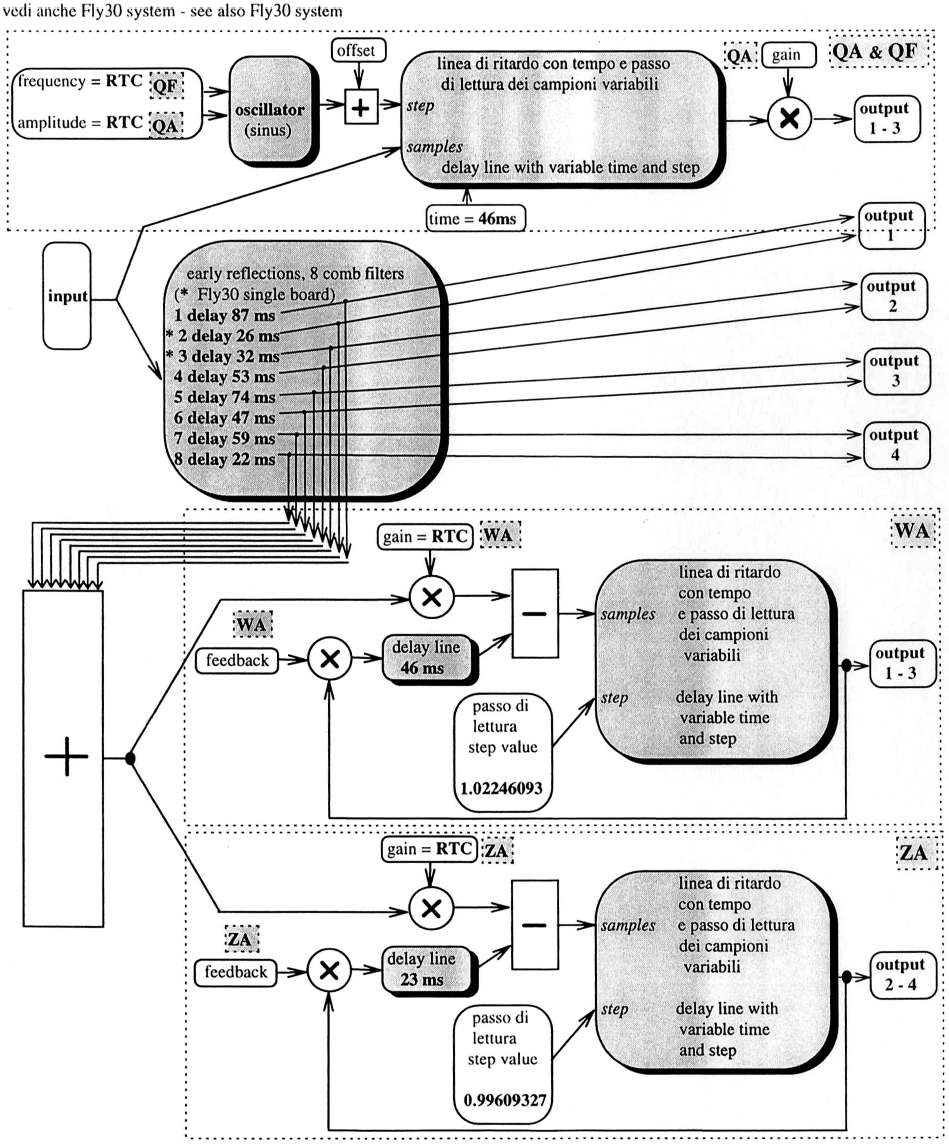
\includegraphics[scale=0.5]{img/1-comp}}
\caption{\label{fft_plot}{\it Ping.}}
\end{figure}

\begin{figure}[ht]
\centerline{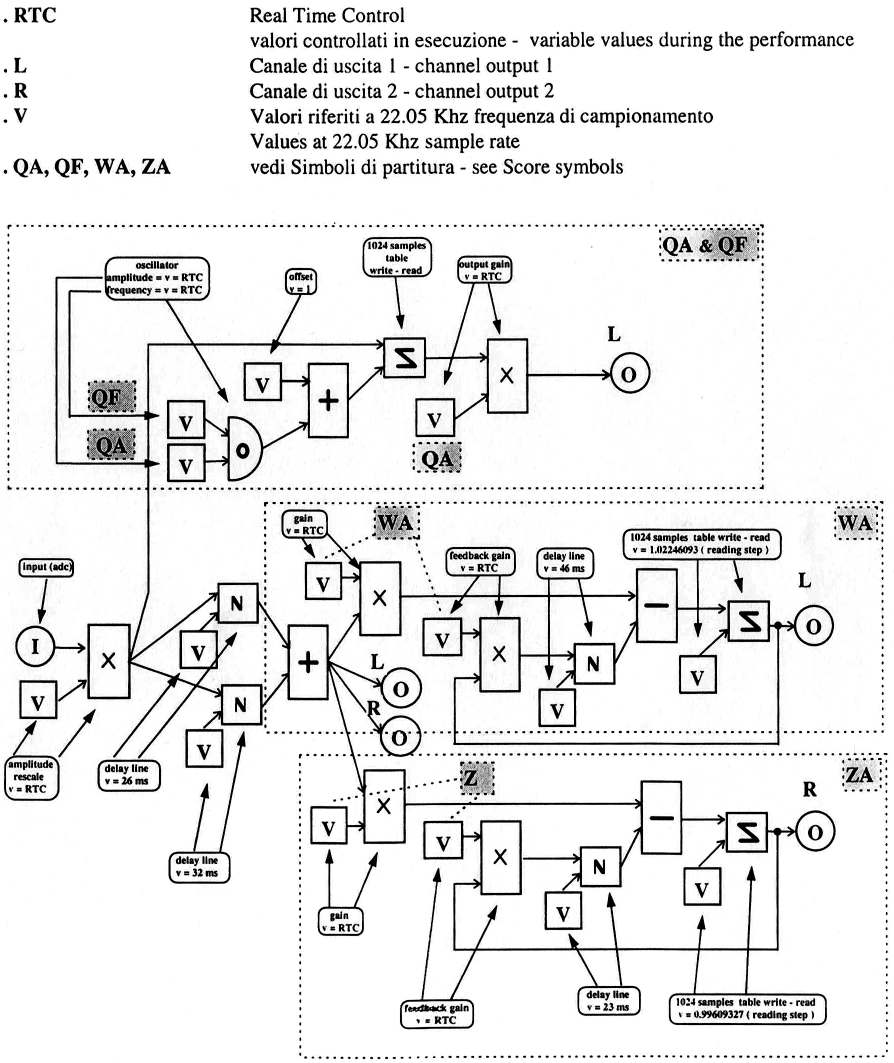
\includegraphics[scale=0.5]{img/2-comp}}
\caption{\label{fft_plot}{\it Ping.}}
\end{figure}

\begin{figure}[ht]
\centerline{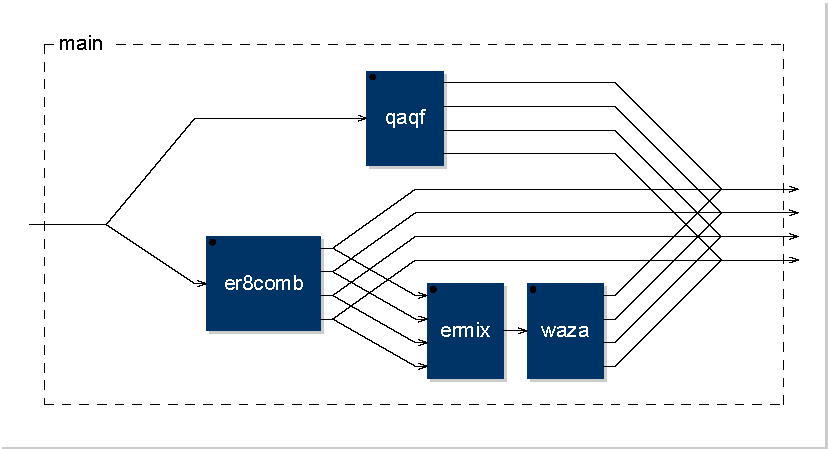
\includegraphics[scale=0.5]{img/main}}
\caption{\label{fft_plot}{\it Ping.}}
\end{figure}

\section{Instruments}
\label{sec:instruments}

Why faust?

Lorem ipsum dolor sit amet, consectetur adipisici elit, sed eiusmod tempor
incidunt ut labore et dolore magna aliqua. Ut enim ad minim veniam, quis
nostrud exercitation ullamco laboris nisi ut aliquid ex ea commodi consequat.
Quis aute iure reprehenderit in voluptate velit esse cillum dolore eu fugiat
nulla pariatur. Excepteur sint obcaecat cupiditat non proident, sunt in culpa
qui officia deserunt mollit anim id est laborum.

%\subsection{Figures}
%\label{ssec:figures}
%
%All figures should be centered on the column (or page, if the figure spans both
%columns). Figure captions (in italic) should follow each figure and have the
%format given in Figure~\ref{fft_plot}. Vectorial figures are preferred (e.g.,
%Postscript, PDF, etc.). Also, in order to provide a better readability, figure
%text font size should be at least identical to footnote font size. If bitmap
%figures are used, please make sure that the resolution is enough for print
%quality. Figure~\ref{ftt_plot2} illustrates an example of a figure spanning two
%columns.

%\begin{figure}[ht]
%\centerline{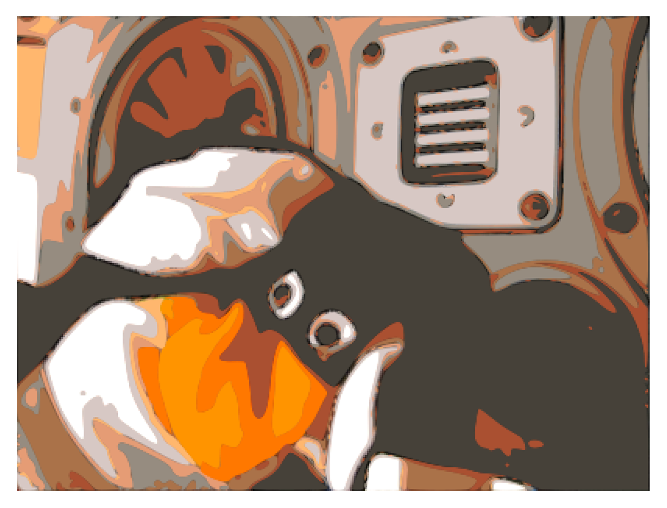
\includegraphics[scale=0.5]{ping}}
%\caption{\label{fft_plot}{\it Ping.}}
%\end{figure}
%
%\begin{figure*}[ht]
%\center
%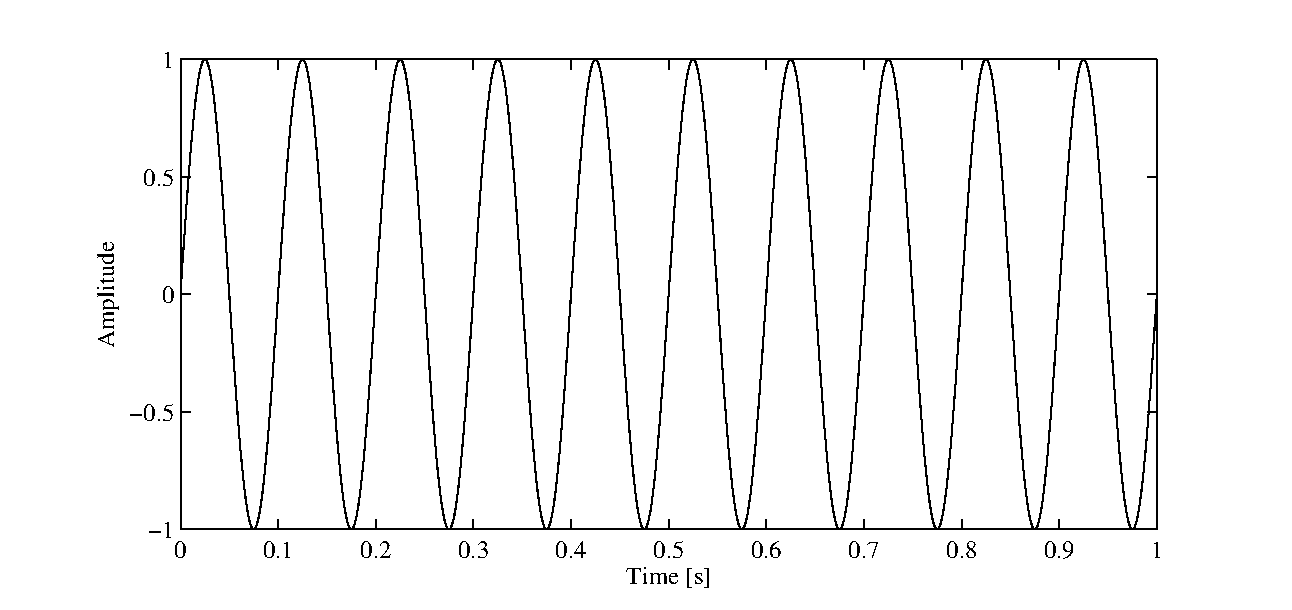
\includegraphics[width=5in]{TwoColumnSine2}
%\caption{\label{ftt_plot2}{\it A figure spanning two columns, as mentioned in
%Sec. \ref{ssec:figures}.}}
%\end{figure*}

%\subsection{Tables}
%
%As for figures, all tables should be centered on the column (or page, if the
%table spans both columns). Table captions should be in italic, precede each
%table and have the format given in Table~\ref{tab:example}.
%
%\begin{table}[ht]
%  \caption{\itshape Basic trigonometric values.}
%	\centering
%	\begin{tabular}{|c|c|}
%		\hline
%		$\mathrm{angle}\,(\theta, \mathrm{rad})$ & $\sin \theta$ \\\hline
%		$\frac{\pi}{2}$ & $1$ \\
%		$\pi$ & $0$ \\
%		$\frac{3\pi}{2}$ & $-1$ \\
%		$2\pi$ & $0$ \\\hline
%	\end{tabular}
%	%
%	\label{tab:example}
%\end{table}
%
%\begin{table*}[ht]
%  \caption{{\it Basic trigonometric values, spanning two columns.}}
%	\centering
%  \begin{tabular}{|c|c|c|c|c|c|c|}\hline
%    $\mathrm{angle}\, (\theta, \mathrm{rad})$ & $\sin \theta$ & $\cos \theta $ & $(\sin \theta)/2 $ & $(\cos \theta) /2 $ & $(\sin \theta)/3 $ & $(\cos \theta)/3$    \\\hline
%    $\frac{\pi}{2}$ & $1$ & $0$ & $1/2$ & $0$ & $1/3$ & $0$ \\
%    $\pi$ & $0$ & $-1$ & $0$ & $-1/2$ & $0$ & $-1/3$\\
%    $\frac{3\pi}{2}$ & $-1$ & $0$ & $-1/2$ & $0$ & $-1/3$ & $0$ \\
%    $2\pi$ & $0$ & $1$ & $0$ & $1/2$ & $0$ & $1/3$ \\\hline
% \end{tabular}
%	%
%  \label{tab:example2}
%\end{table*}
%
%\subsection{Equations}
%
%Equations should be placed on separate lines and numbered:
%
%\begin{equation}
%	y(n)=b_0x(n)-a_1y(n-1)
%	\label{eq1}
%	\end{equation}
%	where equation (\ref{eq1}) is a one pole filter with frequency response:
%	\begin{equation}
%	H(e^{j \omega T}) = \frac{b_0}{1+a_1e^{-j \omega T}}
%	\label{eq2}
%\end{equation}

%\subsection{Code}
%
%Code can be listed in a block:
%
%\begin{lstlisting}
%  int foo = 0;
%\end{lstlisting}
%\noindent
%or directly in-lined in the body of the text: \lstinline{int foo = 1;}.
%
%
%\subsection{References}
%
%The references will be numbered in order of appearance \cite{Sal89},
%\cite{Spa72}, \cite{MosWal64} and \cite{Kay86}. Please avoid listing
%references that do not appear in the text.
%
%\subsubsection{Reference Format}
%
%The reference format is the standard IEEE one. We recommend to use BibTeX to
%create the reference list.

\section{Conclusions}

This template can be found on the conference website. For changing the number
of author affiliations (1 to 4), uncomment the corresponding regions in the
template \texttt{tex} file. Please, submit full-length papers (4 to 8 pages
for full papers and 2 to 4 pages for poster papers) and keep the paper size to
letter (don't change to A4). Submission is fully electronic and automated 
through the Conference Web Submission System. DO NOT send us papers directly by 
e-mail.

%\section{Acknowledgments}
%
%Many thanks to the great number of anonymous reviewers!

%\newpage
\nocite{*}
\bibliographystyle{IEEEbib}
\bibliography{LAC-20} % requires file lac-20.bib

https://www.nytimes.com/1990/03/18/arts/recordings-karajan-vs-karajan-vs-karajan-vs.html

%
%\section{Appendix: Margin Check}
%
%This section shows the column margins for the text.
%
%Lorem ipsum dolor sit amet, consectetur adipisici elit, sed eiusmod tempor
%incidunt ut labore et dolore magna aliqua. Ut enim ad minim veniam, quis
%nostrud exercitation ullamco laboris nisi ut aliquid ex ea commodi consequat.
%Quis aute iure reprehenderit in voluptate velit esse cillum dolore eu fugiat
%nulla pariatur. Excepteur sint obcaecat cupiditat non proident, sunt in culpa
%qui officia deserunt mollit anim id est laborum.

\end{document}
